\begin{figure}[htbp]
\centering
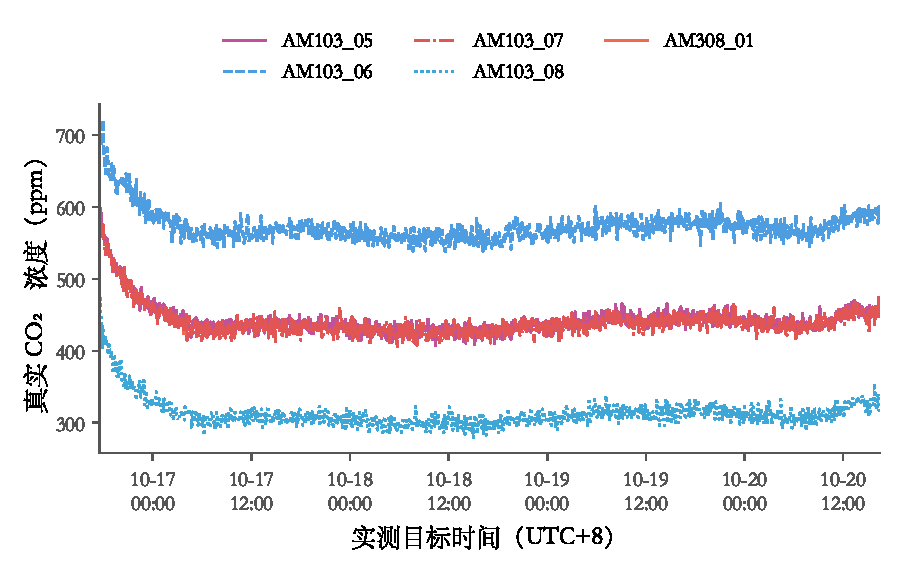
\includegraphics[width=0.85\textwidth]{figures/fig_co2_trend.pdf}
\caption{五个点位的真实 CO₂ 浓度变化}
\end{figure}
\begin{figure}[htbp]
\centering
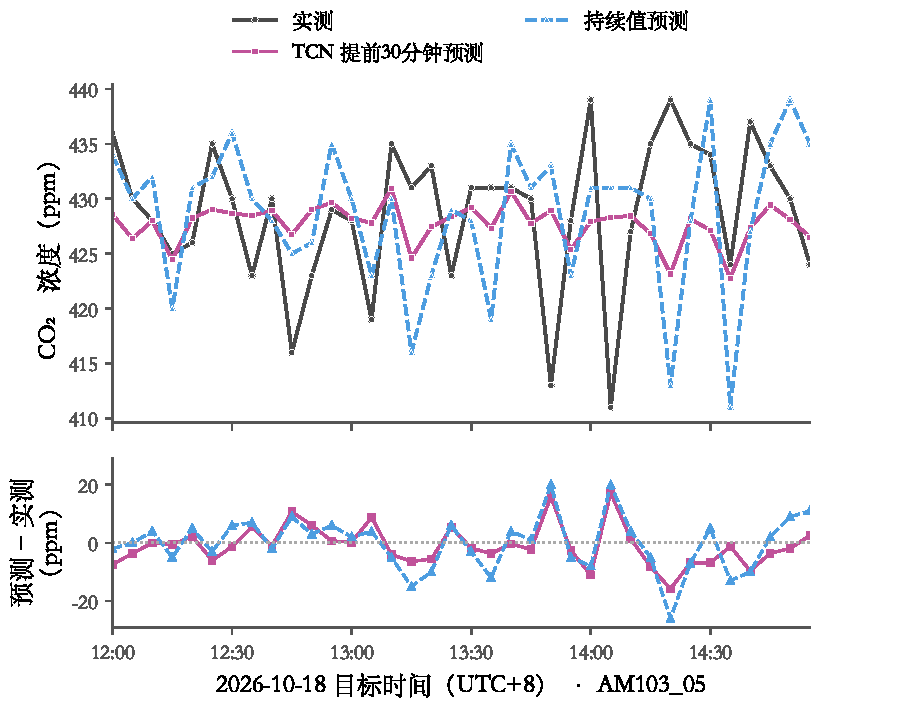
\includegraphics[width=0.85\textwidth]{figures/fig_prediction_overlay.pdf}
\caption{预测与实测，到底贴得多近？}
\end{figure}
\begin{figure}[htbp]
\centering
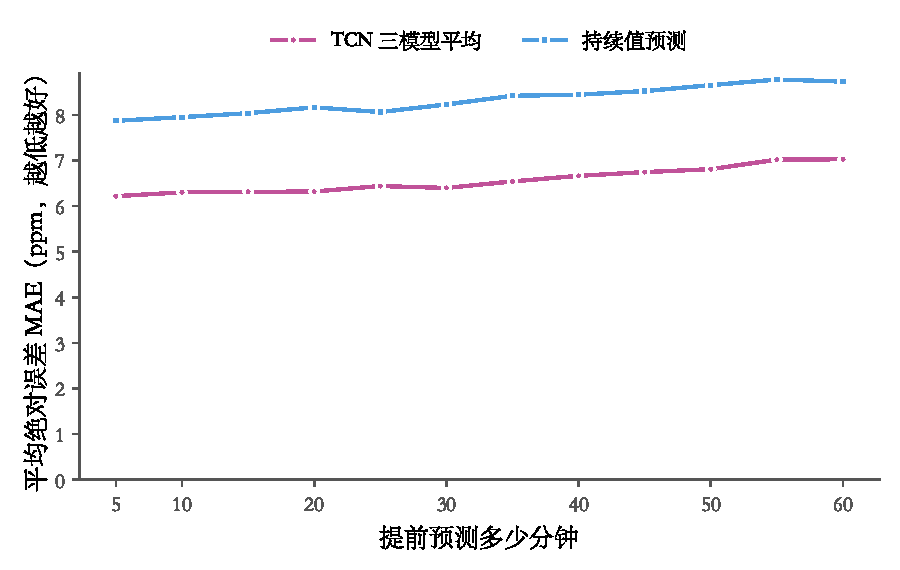
\includegraphics[width=0.85\textwidth]{figures/fig_horizon_error.pdf}
\caption{提前5分钟到60分钟，误差怎么变？}
\end{figure}
\begin{figure}[htbp]
\centering
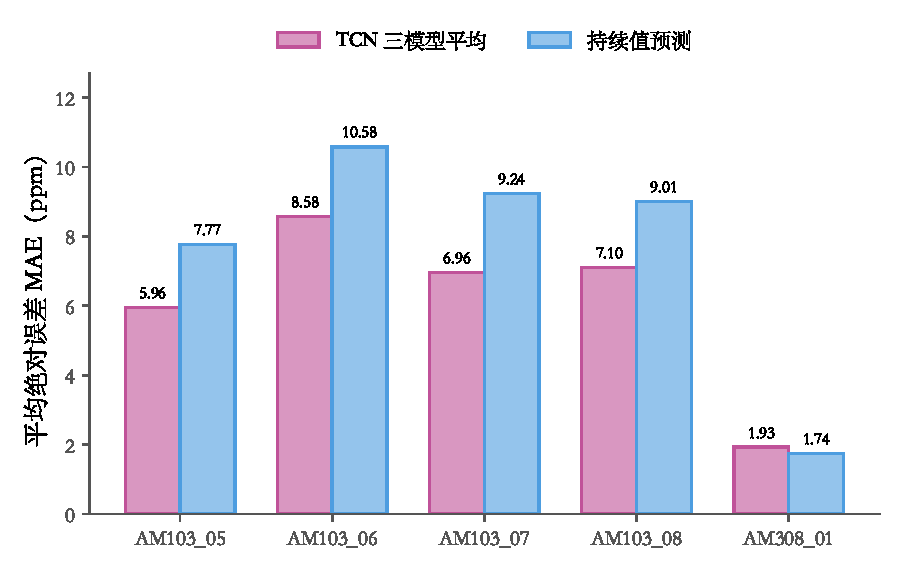
\includegraphics[width=0.85\textwidth]{figures/fig_sensor_error.pdf}
\caption{每个传感器，谁预测得更好？}
\end{figure}
\begin{figure}[htbp]
\centering
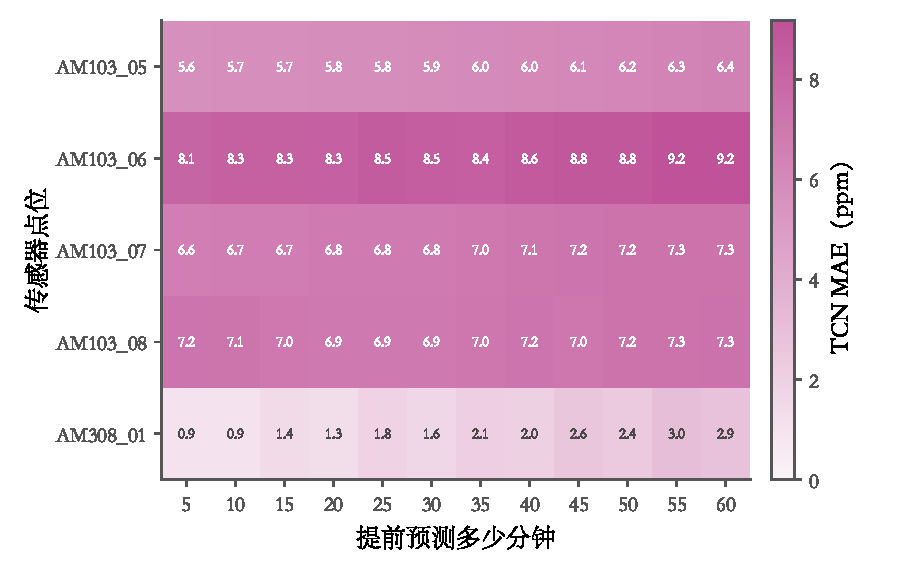
\includegraphics[width=0.85\textwidth]{figures/fig_error_heatmap.pdf}
\caption{哪个点位、哪个预测时距更难？}
\end{figure}
\begin{figure}[htbp]
\centering
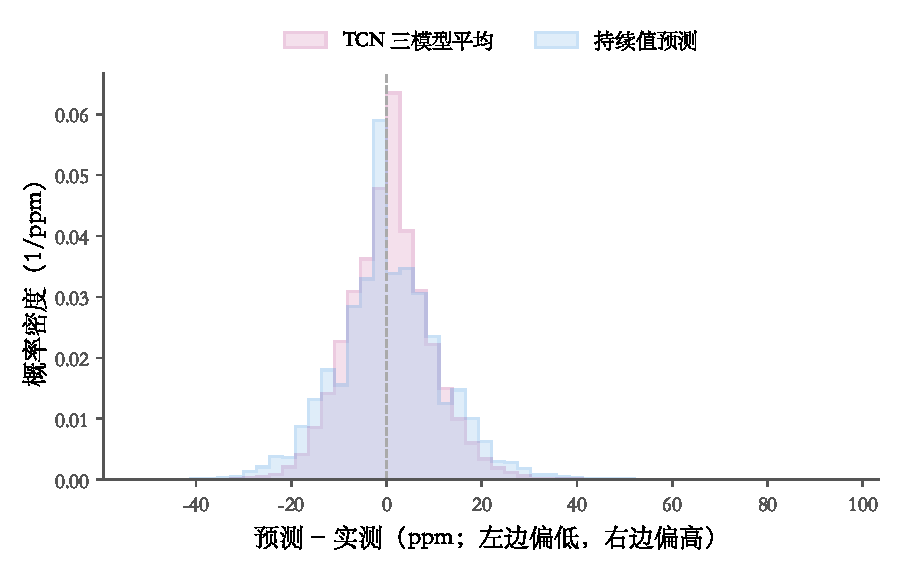
\includegraphics[width=0.85\textwidth]{figures/fig_residual_distribution.pdf}
\caption{模型经常猜高，还是猜低？}
\end{figure}
\begin{figure}[htbp]
\centering
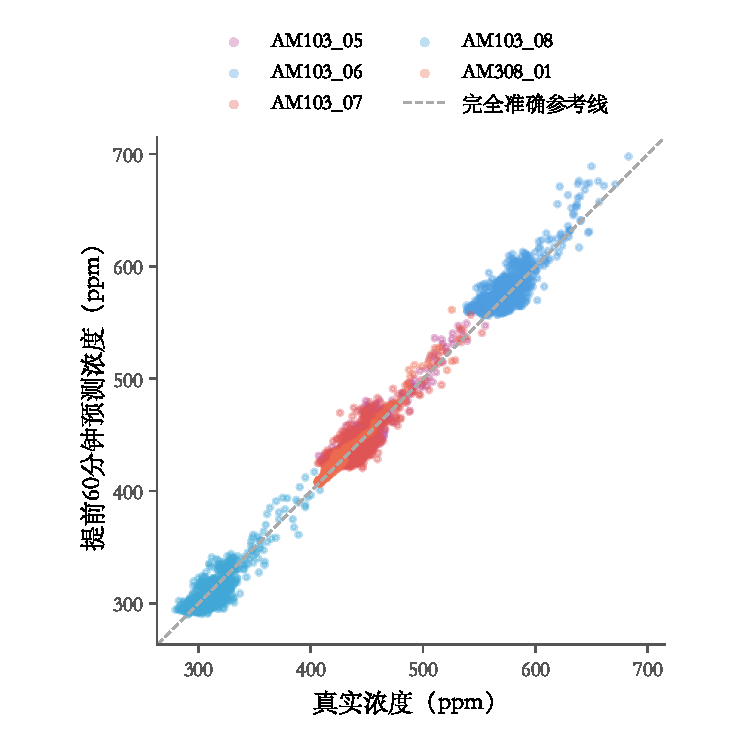
\includegraphics[width=0.85\textwidth]{figures/fig_prediction_scatter.pdf}
\caption{提前一小时的预测，和实测是否一致？}
\end{figure}
